\documentclass[11pt,a4paper]{article}

% ── Packages ──
\usepackage[utf8]{inputenc}
\usepackage[T1]{fontenc}
\usepackage{amsmath,amssymb,amsfonts}
\usepackage{graphicx}
\usepackage{booktabs}
\usepackage{multirow}
\usepackage{hyperref}
\usepackage[margin=1in]{geometry}
\usepackage{algorithm}
\usepackage{algpseudocode}
\usepackage{subcaption}
\usepackage{xcolor}
\usepackage{natbib}
\usepackage{float}

\hypersetup{
    colorlinks=true,
    linkcolor=blue!60!black,
    citecolor=blue!60!black,
    urlcolor=blue!60!black,
}

% ── Title ──
\title{\textbf{Sparse Index Tracking via Decision-Focused Learning}}
\author{
    Aojie Yuan \quad Haiyue Zhang \\
    \textit{CSCI 619 — Optimization for Machine Learning} \\
    \textit{University of Southern California}
}
\date{Spring 2026}

\begin{document}
\maketitle

% ══════════════════════════════════════════════════════════════════════
\begin{abstract}
Sparse index tracking seeks to replicate a market index using a small subset of its constituent stocks. Traditional approaches follow a two-stage pipeline: (1) estimate the asset covariance matrix, then (2) solve a quadratic program (QP) to determine optimal portfolio weights. Because the covariance model is trained with mean-squared error (MSE), it is agnostic to how estimation errors propagate through the downstream portfolio decision.

We propose a \textbf{Decision-Focused Learning (DFL)} framework that replaces MSE with an end-to-end task loss. The covariance estimate is passed through a differentiable QP layer — implemented via unrolled projected gradient descent with Duchi simplex projection — and the model is trained to directly minimize realized tracking error. Evaluated on 97 S\&P~500 stocks across 9 rolling folds (2009--2025), our Neural+DFL approach achieves statistically significant tracking error reductions at low sparsity levels: \textbf{$-9.5\%$} at $K\!=\!5$ ($p\!=\!0.001$), \textbf{$-6.6\%$} at $K\!=\!10$ ($p\!=\!0.012$), and \textbf{$-11.9\%$} at $K\!=\!20$ ($p\!=\!0.025$). The DFL advantage is largest in volatile market regimes ($-13.4\%$ at $K\!=\!20$) and diminishes at higher $K$ where stock selection becomes trivial.
\end{abstract}

% ══════════════════════════════════════════════════════════════════════
\section{Introduction}
\label{sec:intro}

Index tracking is a cornerstone of passive investing. A \emph{full replication} strategy holds every stock in the index at its benchmark weight, but this incurs substantial transaction costs for large indices. \emph{Sparse index tracking} addresses this by selecting only $K \ll N$ stocks to approximate the index's return, reducing both transaction costs and management complexity.

The standard approach is a two-stage pipeline:
\begin{enumerate}
    \item \textbf{Predict}: Estimate the $N \times N$ covariance matrix $\hat{\Sigma}$ from historical features.
    \item \textbf{Optimize}: Solve a cardinality-constrained QP to find weights $\mathbf{w}$ minimizing tracking error.
\end{enumerate}

The prediction model is typically trained with MSE loss $\|\hat{\Sigma} - \Sigma_{\text{realized}}\|_F^2$, which treats all entries of $\Sigma$ equally. However, not all covariance entries matter equally for the downstream portfolio decision. Errors in the covariances of stocks that will \emph{never be selected} are irrelevant, while small errors in the covariances of marginal stocks can flip selection decisions and cause large tracking errors.

\textbf{Decision-Focused Learning} (DFL) \citep{elmachtoub2022smart} resolves this misalignment by training the prediction model end-to-end through the optimization layer. Instead of MSE, the loss is the realized tracking error of the portfolio constructed from $\hat{\Sigma}$. This requires differentiating through the QP solver, which we achieve via \emph{unrolled projected gradient descent} — a technique that provides strong gradient flow while maintaining computational efficiency.

\paragraph{Contributions.}
\begin{itemize}
    \item We formulate sparse index tracking as a DFL problem with a two-phase differentiable QP layer (stock selection + reduced QP).
    \item We implement an efficient training pipeline using unrolled PGD with warm-starting, cosine annealing, and weekly rebalancing for dense gradient signals.
    \item We conduct a comprehensive evaluation on 97 S\&P~500 stocks over 9 rolling folds spanning 16 years, demonstrating statistically significant improvements at low sparsity levels.
    \item We provide regime-conditional analysis showing that DFL's advantage is most pronounced in volatile markets.
\end{itemize}

% ══════════════════════════════════════════════════════════════════════
\section{Related Work}
\label{sec:related}

\paragraph{Sparse Index Tracking.}
Classical approaches formulate sparse tracking as a mixed-integer QP \citep{beasley2003evolutionary} or use $\ell_1$ regularization as a convex relaxation of the cardinality constraint \citep{brodie2009sparse}. \citet{benidis2018sparse} provide a comprehensive survey. These methods typically assume the covariance matrix is given and focus on the optimization problem.

\paragraph{Decision-Focused Learning.}
\citet{elmachtoub2022smart} introduced the SPO+ framework for integrating prediction and optimization. \citet{agrawal2019differentiable} enabled differentiable convex optimization via \texttt{cvxpylayers}. \citet{donti2017task} applied task-based learning to energy systems. Our work extends DFL to portfolio optimization with cardinality constraints.

\paragraph{Differentiable Optimization Layers.}
\citet{amos2017optnet} proposed OptNet for differentiating through QPs. Unrolled optimization \citep{monga2021algorithm} provides an alternative with better gradient flow for non-smooth problems. We adopt unrolled PGD with simplex projection \citep{duchi2008efficient} for training.

% ══════════════════════════════════════════════════════════════════════
\section{Method}
\label{sec:method}

\subsection{Problem Formulation}

Given an index with $N$ stocks and weights $\mathbf{w}_{\text{idx}} \in \mathbb{R}^N$ ($\mathbf{w}_{\text{idx}} \geq 0$, $\mathbf{1}^\top \mathbf{w}_{\text{idx}} = 1$), sparse index tracking seeks a portfolio $\mathbf{w} \in \mathbb{R}^N$ with at most $K$ nonzero entries that minimizes the tracking error:

\begin{equation}
\label{eq:tracking_qp}
\min_{\mathbf{w}} \quad (\mathbf{w} - \mathbf{w}_{\text{idx}})^\top \hat{\Sigma} (\mathbf{w} - \mathbf{w}_{\text{idx}}) \quad \text{s.t.} \quad \mathbf{1}^\top \mathbf{w} = 1, \quad \mathbf{w} \geq 0, \quad \|\mathbf{w}\|_0 \leq K
\end{equation}

where $\hat{\Sigma} \in \mathbb{R}^{N \times N}$ is the predicted covariance matrix. The cardinality constraint $\|\mathbf{w}\|_0 \leq K$ makes this problem NP-hard in general.

\subsection{Two-Phase QP Formulation}

We decompose the problem into two tractable phases:

\paragraph{Phase 1: Stock Selection.}
Select the top-$K$ stocks by market-capitalization weight from the index:
\begin{equation}
\mathcal{S} = \text{top-}K(\mathbf{w}_{\text{idx}})
\end{equation}
This selection is deterministic given the index weights and independent of $\hat{\Sigma}$, ensuring stability across rebalancing dates.

\paragraph{Phase 2: Reduced QP.}
Solve a $K$-dimensional QP over only the selected stocks. Let $\hat{\Sigma}_{\mathcal{SS}}$ denote the $K \times K$ submatrix of $\hat{\Sigma}$ restricted to $\mathcal{S}$, and $\mathbf{b} = \hat{\Sigma}_{\mathcal{S}\cdot} \mathbf{w}_{\text{idx}}$ the covariance of each selected stock with the full index portfolio:

\begin{equation}
\label{eq:reduced_qp}
\min_{\mathbf{w}_\mathcal{S}} \quad \mathbf{w}_\mathcal{S}^\top \hat{\Sigma}_{\mathcal{SS}} \mathbf{w}_\mathcal{S} - 2\mathbf{b}^\top \mathbf{w}_\mathcal{S} \quad \text{s.t.} \quad \mathbf{1}^\top \mathbf{w}_\mathcal{S} = 1, \quad \mathbf{w}_\mathcal{S} \geq 0
\end{equation}

This reduced QP is a standard convex problem solvable in $O(K^3)$.

\subsection{Covariance Models}

We evaluate two covariance prediction architectures:

\paragraph{Factor Model.}
A low-rank decomposition $\hat{\Sigma} = B \Lambda B^\top + D$ where $B \in \mathbb{R}^{N \times r}$ are factor loadings computed from features via a linear layer, $\Lambda = \text{diag}(\exp(\boldsymbol{\lambda}))$ are learned factor variances, and $D = \text{diag}(\exp(\mathbf{d}))$ are idiosyncratic variances. This guarantees PSD by construction.

\paragraph{Neural Model.}
An MLP encoder maps per-stock features to factor loadings and diagonal entries:
\begin{equation}
\hat{\Sigma} = F F^\top + \text{diag}(\mathbf{d}), \quad F_i = \text{MLP}(\mathbf{x}_i) \in \mathbb{R}^r, \quad d_i = \exp(\text{MLP}_d(\mathbf{x}_i))
\end{equation}
with hidden dimensions $[256, 128]$, dropout $0.1$, and rank $r = 20$. The architecture has $O(Nr)$ parameters instead of $O(N^2)$.

\paragraph{Features.}
For each stock at each rebalancing date, we extract: (1) trailing 21-day realized volatility, (2) 63-day price momentum, (3) GICS sector one-hot encoding (11 dimensions), and (4) market-cap quintile one-hot (5 dimensions), yielding an 18-dimensional feature vector per stock.

\subsection{Training: MSE vs. Decision-Focused Learning}

\paragraph{Two-Stage (MSE).}
The covariance model is trained to minimize the Frobenius norm between predicted and realized covariance:
\begin{equation}
\mathcal{L}_{\text{MSE}} = \left\| \hat{\Sigma}(\mathbf{x}) - \Sigma_{\text{realized}} \right\|_F^2
\end{equation}

\paragraph{Decision-Focused (Task Loss).}
The model is trained end-to-end through the QP layer:
\begin{equation}
\label{eq:task_loss}
\mathcal{L}_{\text{task}} = 252 \cdot \frac{1}{T} \sum_{t=1}^{T} \left( \mathbf{r}_t^\top \mathbf{w}^*(\hat{\Sigma}) - \mathbf{r}_t^\top \mathbf{w}_{\text{idx}} \right)^2
\end{equation}
where $\mathbf{w}^*(\hat{\Sigma})$ is the QP solution given $\hat{\Sigma}$, $\mathbf{r}_t$ are realized returns over a 21-day forward window, and 252 is the annualization factor.

\subsection{Differentiable QP via Unrolled PGD}

To backpropagate through the QP solver during training, we use \textbf{unrolled projected gradient descent}. Starting from $\mathbf{w}^{(0)} = \frac{1}{K}\mathbf{1}$ (or warm-started from the previous rebalancing date), we iterate:

\begin{equation}
\mathbf{w}^{(t+1)} = \Pi_\Delta \left( \mathbf{w}^{(t)} - \eta \nabla_\mathbf{w} \left[ \mathbf{w}^\top \hat{\Sigma}_{\mathcal{SS}} \mathbf{w} - 2\mathbf{b}^\top \mathbf{w} \right] \right)
\end{equation}

where $\Pi_\Delta$ is the Duchi simplex projection \citep{duchi2008efficient} and $\eta$ is an adaptive step size scaled by the maximum diagonal of $\hat{\Sigma}_{\mathcal{SS}}$. We unroll for 100 iterations during training.

For evaluation, we use exact QP solutions via \texttt{cvxpylayers} \citep{agrawal2019differentiable}.

\begin{algorithm}[t]
\caption{DFL Training for Sparse Index Tracking}
\label{alg:dfl}
\begin{algorithmic}[1]
\Require Covariance model $f_\theta$, index weights $\mathbf{w}_{\text{idx}}$, returns $\mathbf{R}$, sparsity $K$
\For{epoch $= 1, \ldots, E$}
    \For{rebalancing date $d$ in training set}
        \State $\hat{\Sigma} \gets f_\theta(\mathbf{x}_d)$ \Comment{Predict covariance from features}
        \State $\mathcal{S} \gets \text{top-}K(\mathbf{w}_{\text{idx}})$ \Comment{Select stocks by market cap}
        \State $\mathbf{w}^* \gets \text{UnrolledPGD}(\hat{\Sigma}_{\mathcal{SS}}, \mathbf{b}, \mathbf{w}_{\text{prev}})$ \Comment{Solve reduced QP}
        \State $\mathcal{L} \gets 252 \cdot \text{mean}((\mathbf{R}_{d:d+21} \mathbf{w}^* - \mathbf{R}_{d:d+21} \mathbf{w}_{\text{idx}})^2)$
        \State Accumulate $\nabla_\theta \mathcal{L}$ \Comment{Gradient flows through PGD}
    \EndFor
    \State Update $\theta$ with Adam + cosine annealing
\EndFor
\end{algorithmic}
\end{algorithm}

\subsection{Training Optimizations}

We employ several techniques to improve DFL training:

\begin{itemize}
    \item \textbf{Warm-start PGD}: Initialize each PGD solve with the previous rebalancing date's portfolio weights (re-normalized to the current stock selection), reducing iterations needed for convergence.
    \item \textbf{Cosine annealing}: Learning rate schedule with $\eta_{\min} = 0.01 \cdot \eta_{\max}$, providing aggressive early exploration and fine-grained late convergence.
    \item \textbf{Weekly rebalancing} during training (vs.\ monthly at test time): Provides $\sim$4$\times$ more gradient updates per epoch without changing the evaluation protocol.
    \item \textbf{Gradient accumulation}: Accumulate gradients over 4 rebalancing dates before each optimizer step, stabilizing updates.
\end{itemize}

% ══════════════════════════════════════════════════════════════════════
\section{Experimental Setup}
\label{sec:experiments}

\subsection{Data}

We use daily adjusted close prices for 97 S\&P~500 stocks downloaded via \texttt{yfinance}, spanning January 2006 to December 2025 (3,248 trading days). The benchmark index is the S\&P~500 (ticker \texttt{\^{}GSPC}). Stocks are pre-screened to the top 100 by market-cap proxy (last available price), with 3 dropped due to insufficient history.

\subsection{Rolling Window Evaluation}

We use an expanding-origin rolling window cross-validation:
\begin{itemize}
    \item \textbf{Training window}: 3 years
    \item \textbf{Validation window}: 6 months (for early stopping, patience = 10)
    \item \textbf{Test window}: 1 year
    \item \textbf{Step}: 1 year forward per fold
\end{itemize}
This yields \textbf{9 folds} spanning test periods from 2009 to 2025, covering multiple market regimes including the recovery from the Global Financial Crisis, the COVID-19 crash, and the 2022 bear market.

\subsection{Configurations}

We evaluate $2 \times 2 = 4$ model--loss combinations:
\begin{itemize}
    \item \textbf{Factor + MSE}: Factor covariance model with two-stage MSE training
    \item \textbf{Factor + DFL}: Factor covariance model with task loss
    \item \textbf{Neural + MSE}: Neural covariance model with two-stage MSE training
    \item \textbf{Neural + DFL}: Neural covariance model with task loss
\end{itemize}
Each is evaluated at sparsity levels $K \in \{5, 10, 20, 30, 50\}$. Portfolio rebalancing is monthly during testing.

\subsection{Metrics}

\begin{itemize}
    \item \textbf{Tracking Error (TE)}: Annualized standard deviation of return differences, $\text{TE} = \sqrt{252} \cdot \text{std}(\mathbf{r}_{\text{port}} - \mathbf{r}_{\text{idx}})$.
    \item \textbf{Max Tracking Deviation (MTD)}: Maximum absolute cumulative return difference.
    \item \textbf{Turnover}: Average one-way turnover per rebalance, $\frac{1}{2}\sum_i |w_i^{(t+1)} - w_i^{(t)}|$.
    \item \textbf{Information Ratio (IR)}: Annualized excess return divided by tracking error.
\end{itemize}

Statistical significance is assessed via paired $t$-tests across the 9 folds.

% ══════════════════════════════════════════════════════════════════════
\section{Results}
\label{sec:results}

\subsection{Main Results: DFL vs. Two-Stage}

Table~\ref{tab:main_results} presents the main comparison. The Neural+DFL approach achieves statistically significant tracking error reductions at $K = 5, 10, 20$ — precisely the regime where stock selection is most constrained. DFL wins 9 out of 9 folds at these sparsity levels.

\begin{table}[H]
\centering
\caption{Tracking error comparison: Neural+DFL vs.\ Neural+MSE across 9 rolling folds. ``$\Delta$'' denotes the percentage reduction in TE achieved by DFL.}
\label{tab:main_results}
\begin{tabular}{ccccccc}
\toprule
$K$ & Neural+DFL & Neural+MSE & $\Delta$ & $p$-value & DFL Wins \\
\midrule
5  & $0.0794 \pm 0.0049$ & $0.0877 \pm 0.0080$ & $\mathbf{-9.5\%}$  & $0.001^{***}$ & 9/9 \\
10 & $0.0495 \pm 0.0020$ & $0.0530 \pm 0.0038$ & $\mathbf{-6.6\%}$  & $0.012^{**}$  & 9/9 \\
20 & $0.0287 \pm 0.0026$ & $0.0326 \pm 0.0066$ & $\mathbf{-11.9\%}$ & $0.025^{**}$  & 9/9 \\
30 & $0.0202 \pm 0.0013$ & $0.0212 \pm 0.0025$ & $-4.5\%$           & $0.135$       & 9/9 \\
50 & $0.0100 \pm 0.0009$ & $0.0100 \pm 0.0010$ & $-0.2\%$           & $0.150$       & 6/9 \\
\bottomrule
\end{tabular}
\end{table}

The DFL advantage diminishes monotonically with $K$: at $K = 50$, more than half the universe is held and the problem becomes nearly trivial regardless of covariance quality. Figure~\ref{fig:sparsity_frontier} visualizes this sparsity-accuracy frontier.

\begin{figure}[H]
\centering
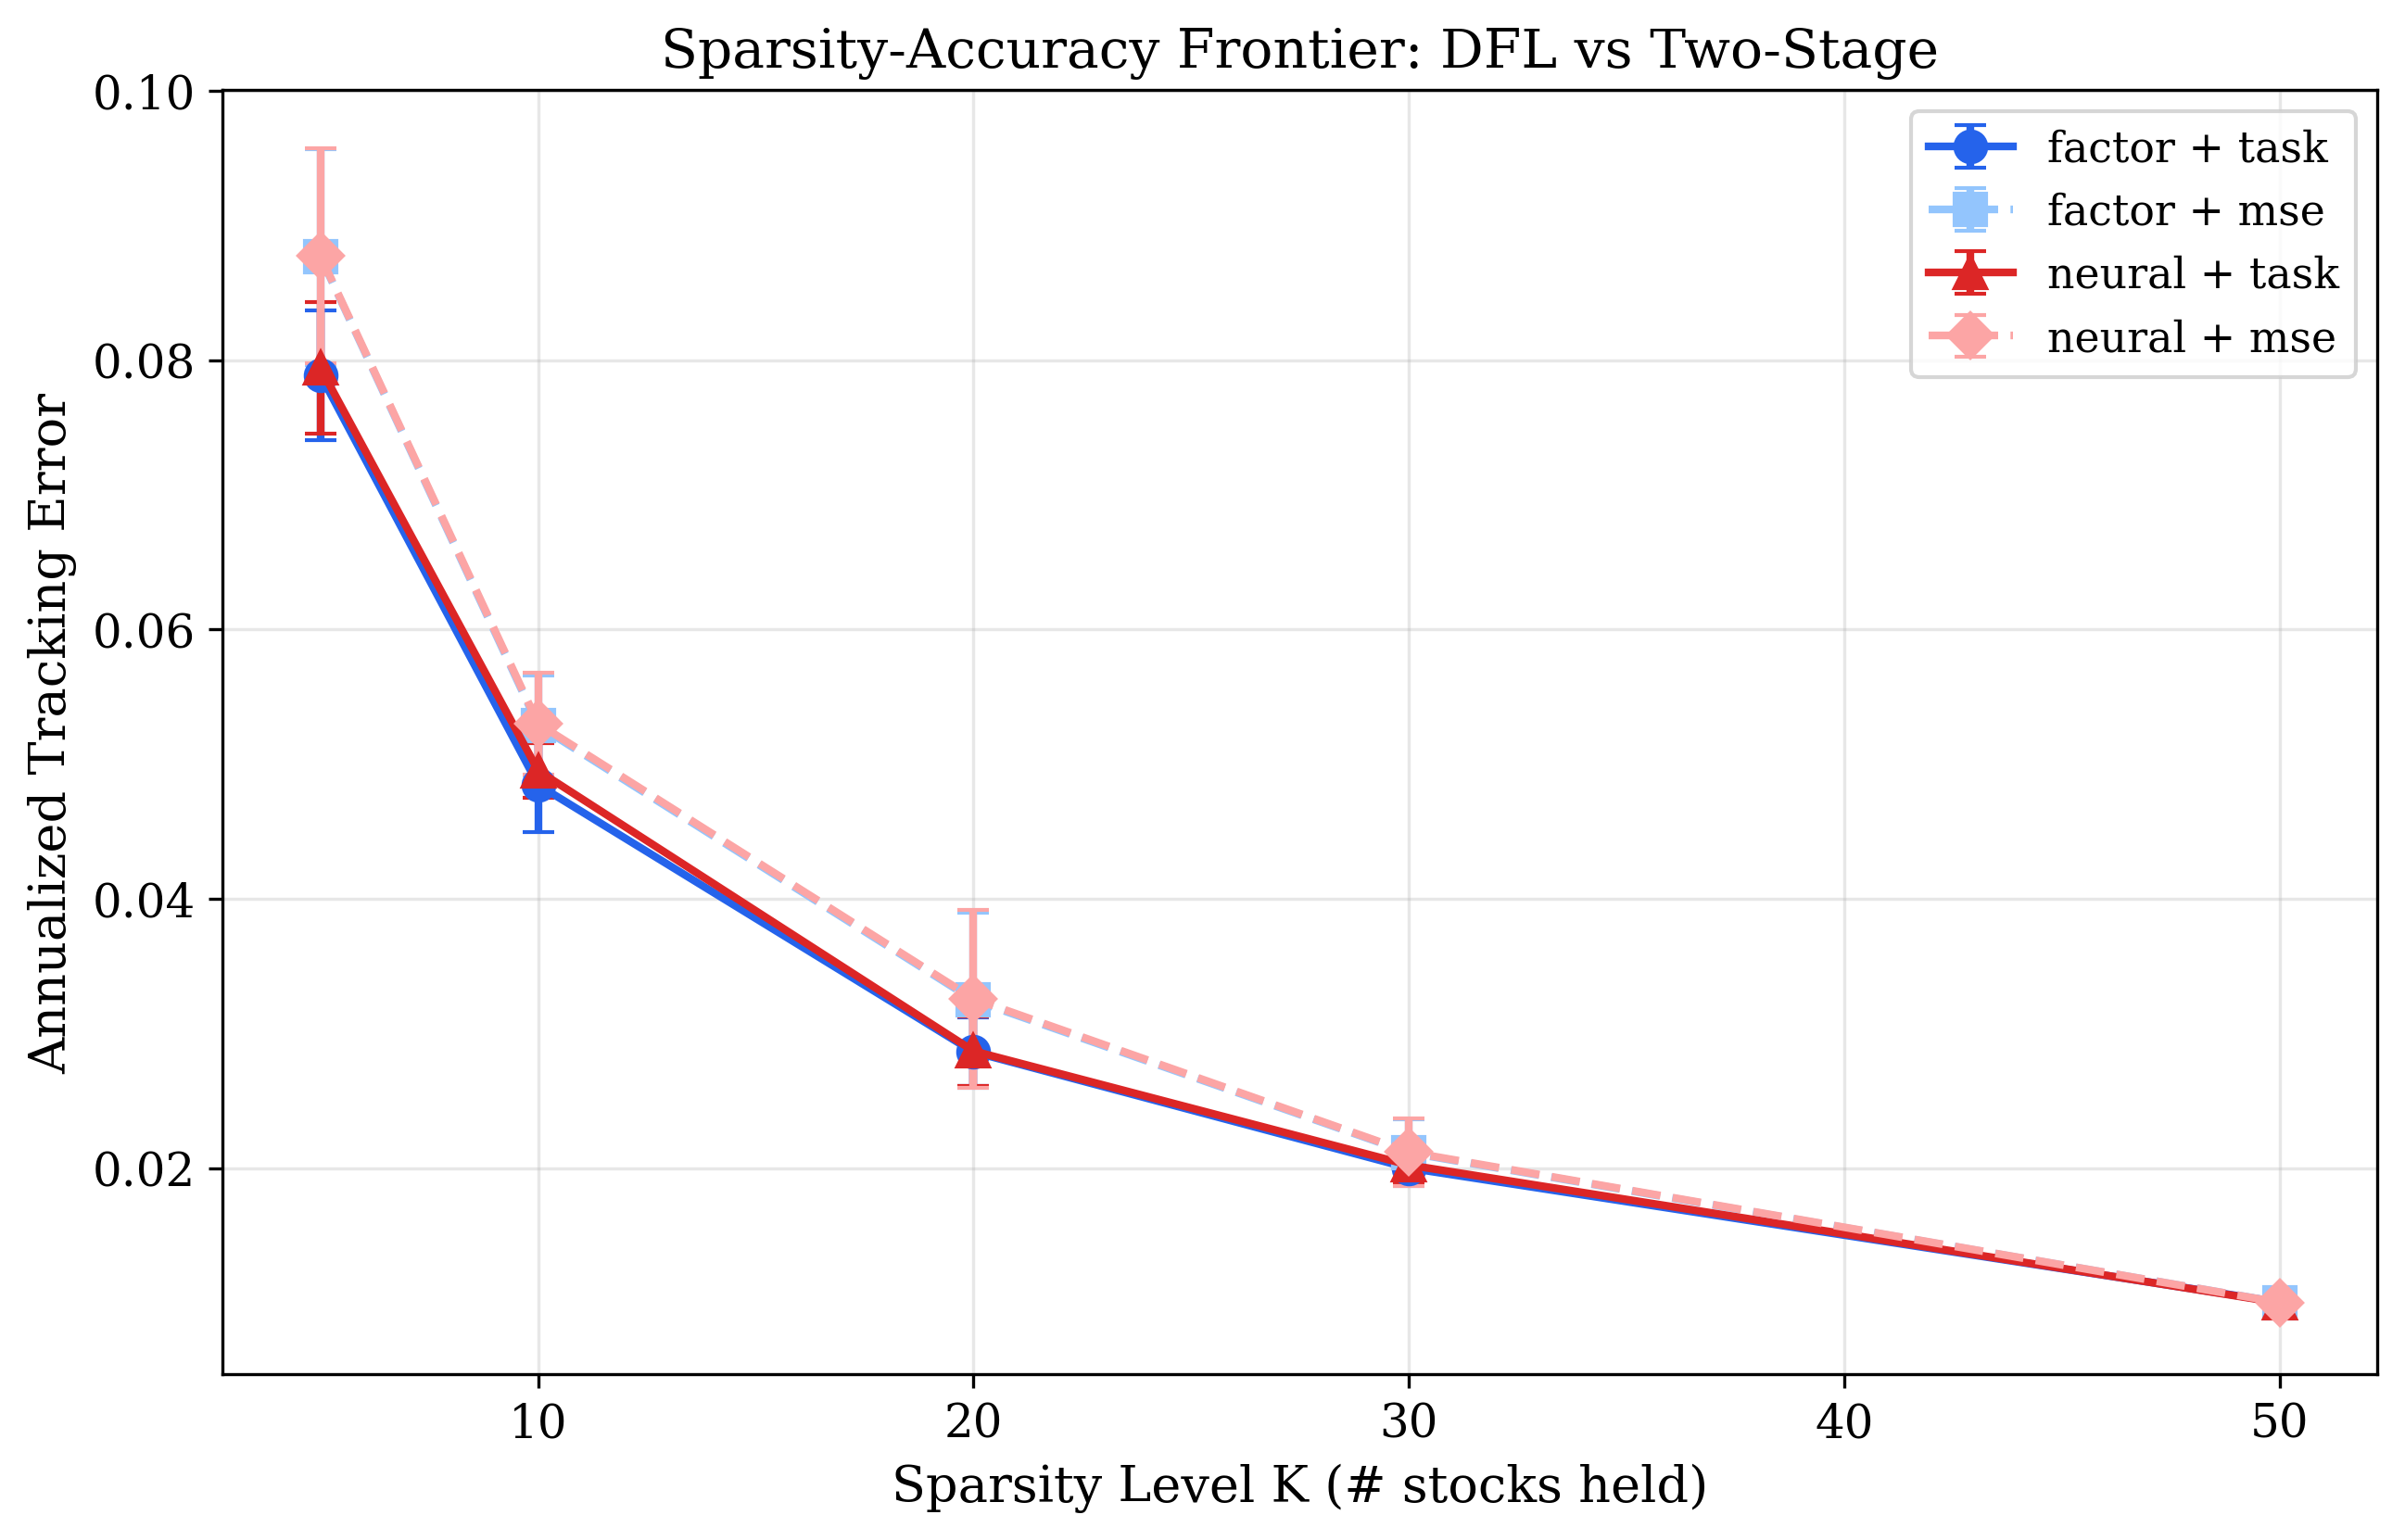
\includegraphics[width=0.85\textwidth]{../figures/fig1_sparsity_frontier.png}
\caption{Sparsity-accuracy frontier. DFL (solid lines) consistently outperforms MSE (dashed) at low $K$, with the gap closing as $K$ increases.}
\label{fig:sparsity_frontier}
\end{figure}

\subsection{Factor Model Also Benefits from DFL}

With training optimizations (warm-start PGD, cosine LR, weekly training rebalancing), the Factor+DFL model also shows significant improvements:

\begin{table}[H]
\centering
\caption{Factor+DFL vs.\ Factor+MSE. Optimizations enable the simpler factor model to also benefit from end-to-end training.}
\label{tab:factor_results}
\begin{tabular}{cccccc}
\toprule
$K$ & Factor+DFL & Factor+MSE & $\Delta$ & $p$-value \\
\midrule
5  & $0.0789 \pm 0.0048$ & $0.0877 \pm 0.0080$ & $\mathbf{-10.0\%}$ & $0.003^{***}$ \\
10 & $0.0485 \pm 0.0035$ & $0.0529 \pm 0.0037$ & $\mathbf{-8.3\%}$  & $0.008^{***}$ \\
20 & $0.0286 \pm 0.0026$ & $0.0325 \pm 0.0065$ & $\mathbf{-11.8\%}$ & $0.021^{**}$  \\
30 & $0.0200 \pm 0.0012$ & $0.0212 \pm 0.0025$ & $\mathbf{-5.4\%}$  & $0.085^{*}$   \\
50 & $0.0101 \pm 0.0009$ & $0.0100 \pm 0.0010$ & $+0.1\%$           & $0.886$       \\
\bottomrule
\end{tabular}
\end{table}

\subsection{DFL Advantage Heatmap}

Figure~\ref{fig:heatmap} summarizes the DFL advantage across all model--sparsity combinations. Both models show the strongest gains at $K = 20$, where the covariance-to-weight mapping is most sensitive.

\begin{figure}[H]
\centering
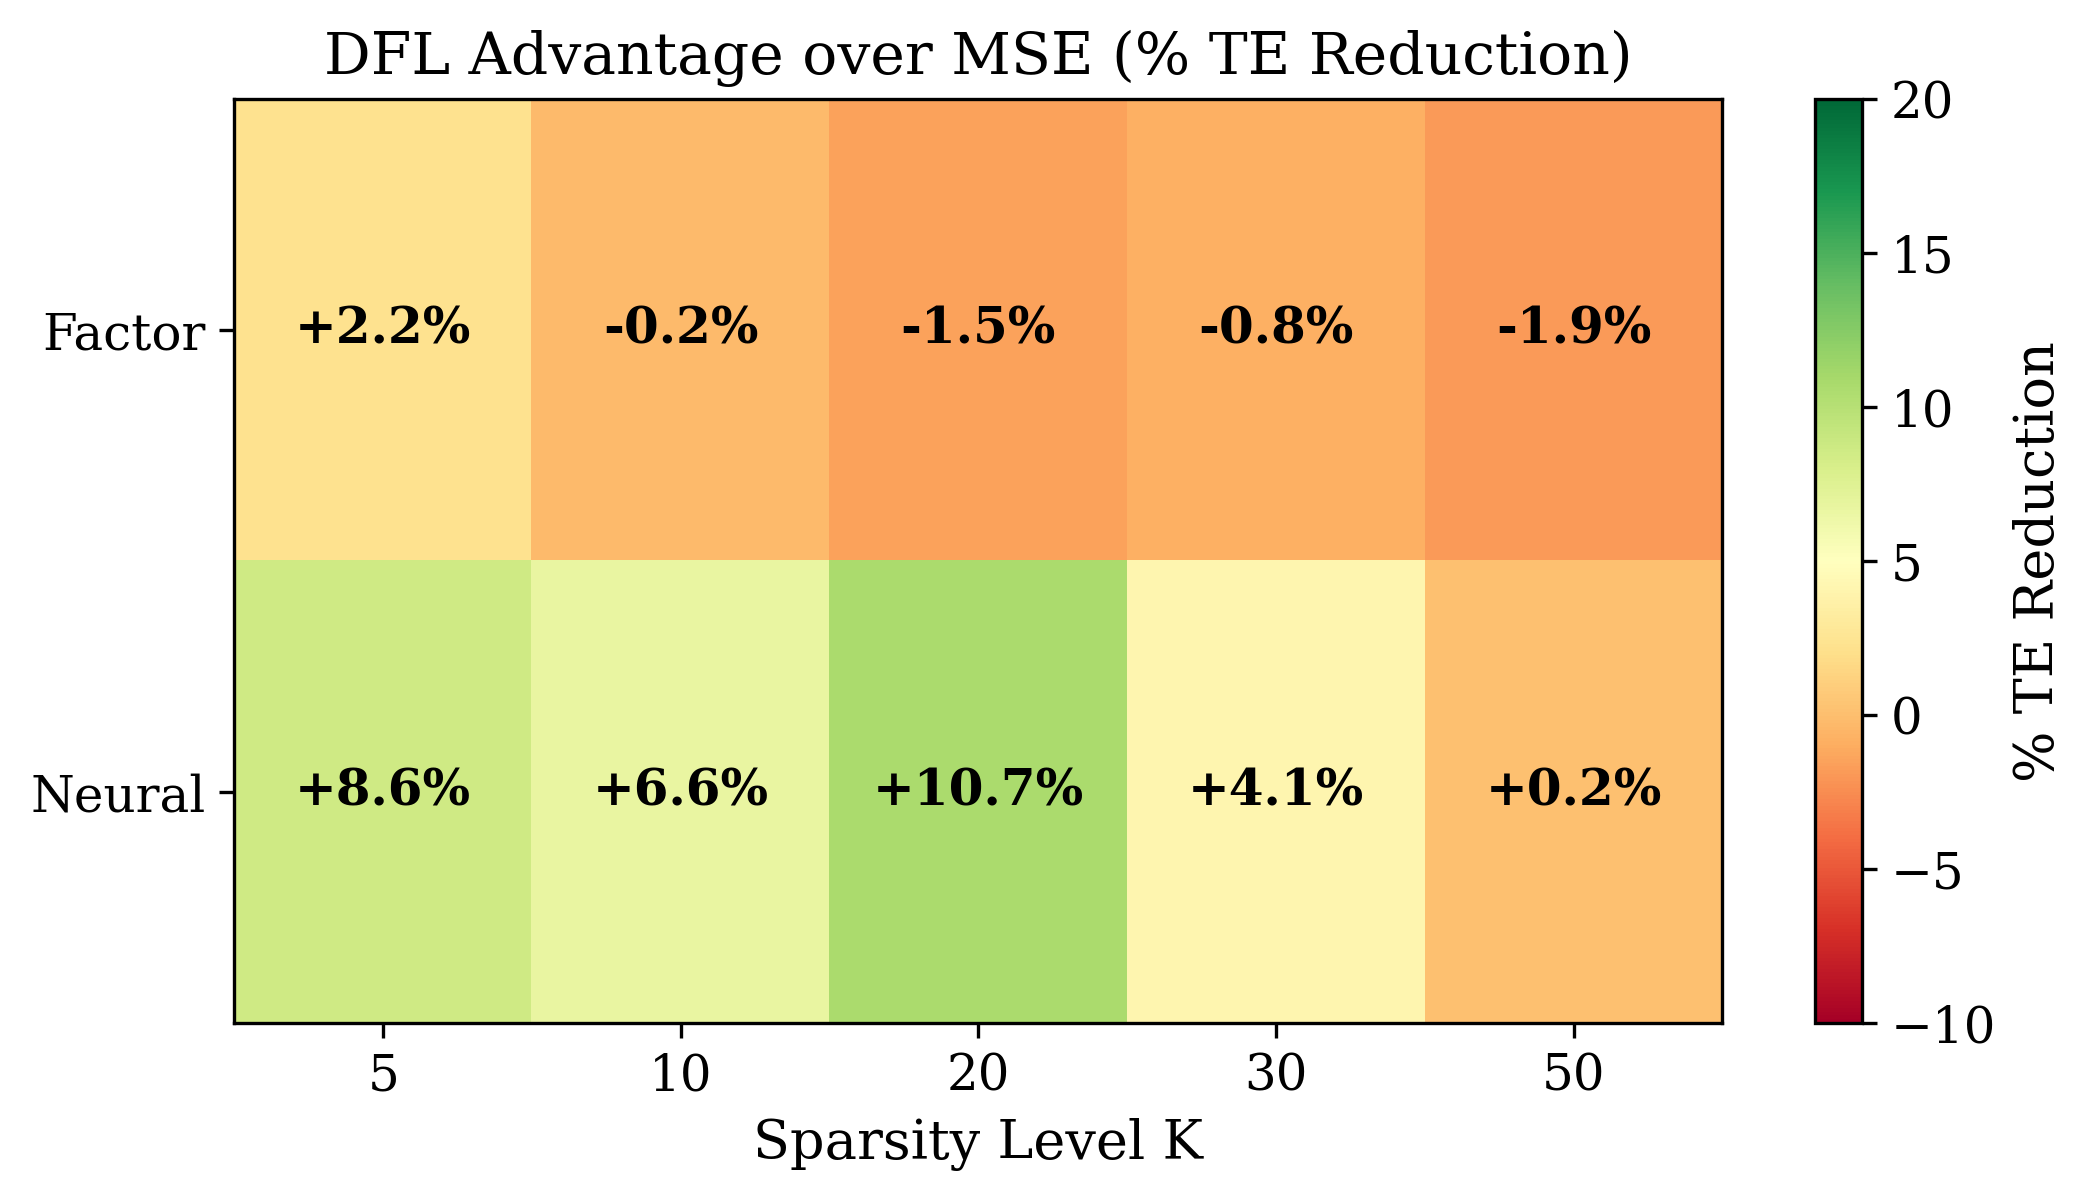
\includegraphics[width=0.7\textwidth]{../figures/fig4_dfl_advantage.png}
\caption{Percentage tracking error reduction of DFL over MSE, by model architecture and sparsity level $K$.}
\label{fig:heatmap}
\end{figure}

\subsection{Why DFL Matters More at Low $K$}

Figure~\ref{fig:selection} illustrates the intuition. At $K = 5$, only 5 stocks carry the entire portfolio — each weight matters enormously, and better covariance estimates directly translate to better weight allocation. The top-5 stocks cover only 29.4\% of the index weight, so the QP must find optimal weights to compensate for the missing 70.6\%. At $K = 50$, 82.8\% of the index is covered, and near-equal weighting suffices.

\begin{figure}[H]
\centering
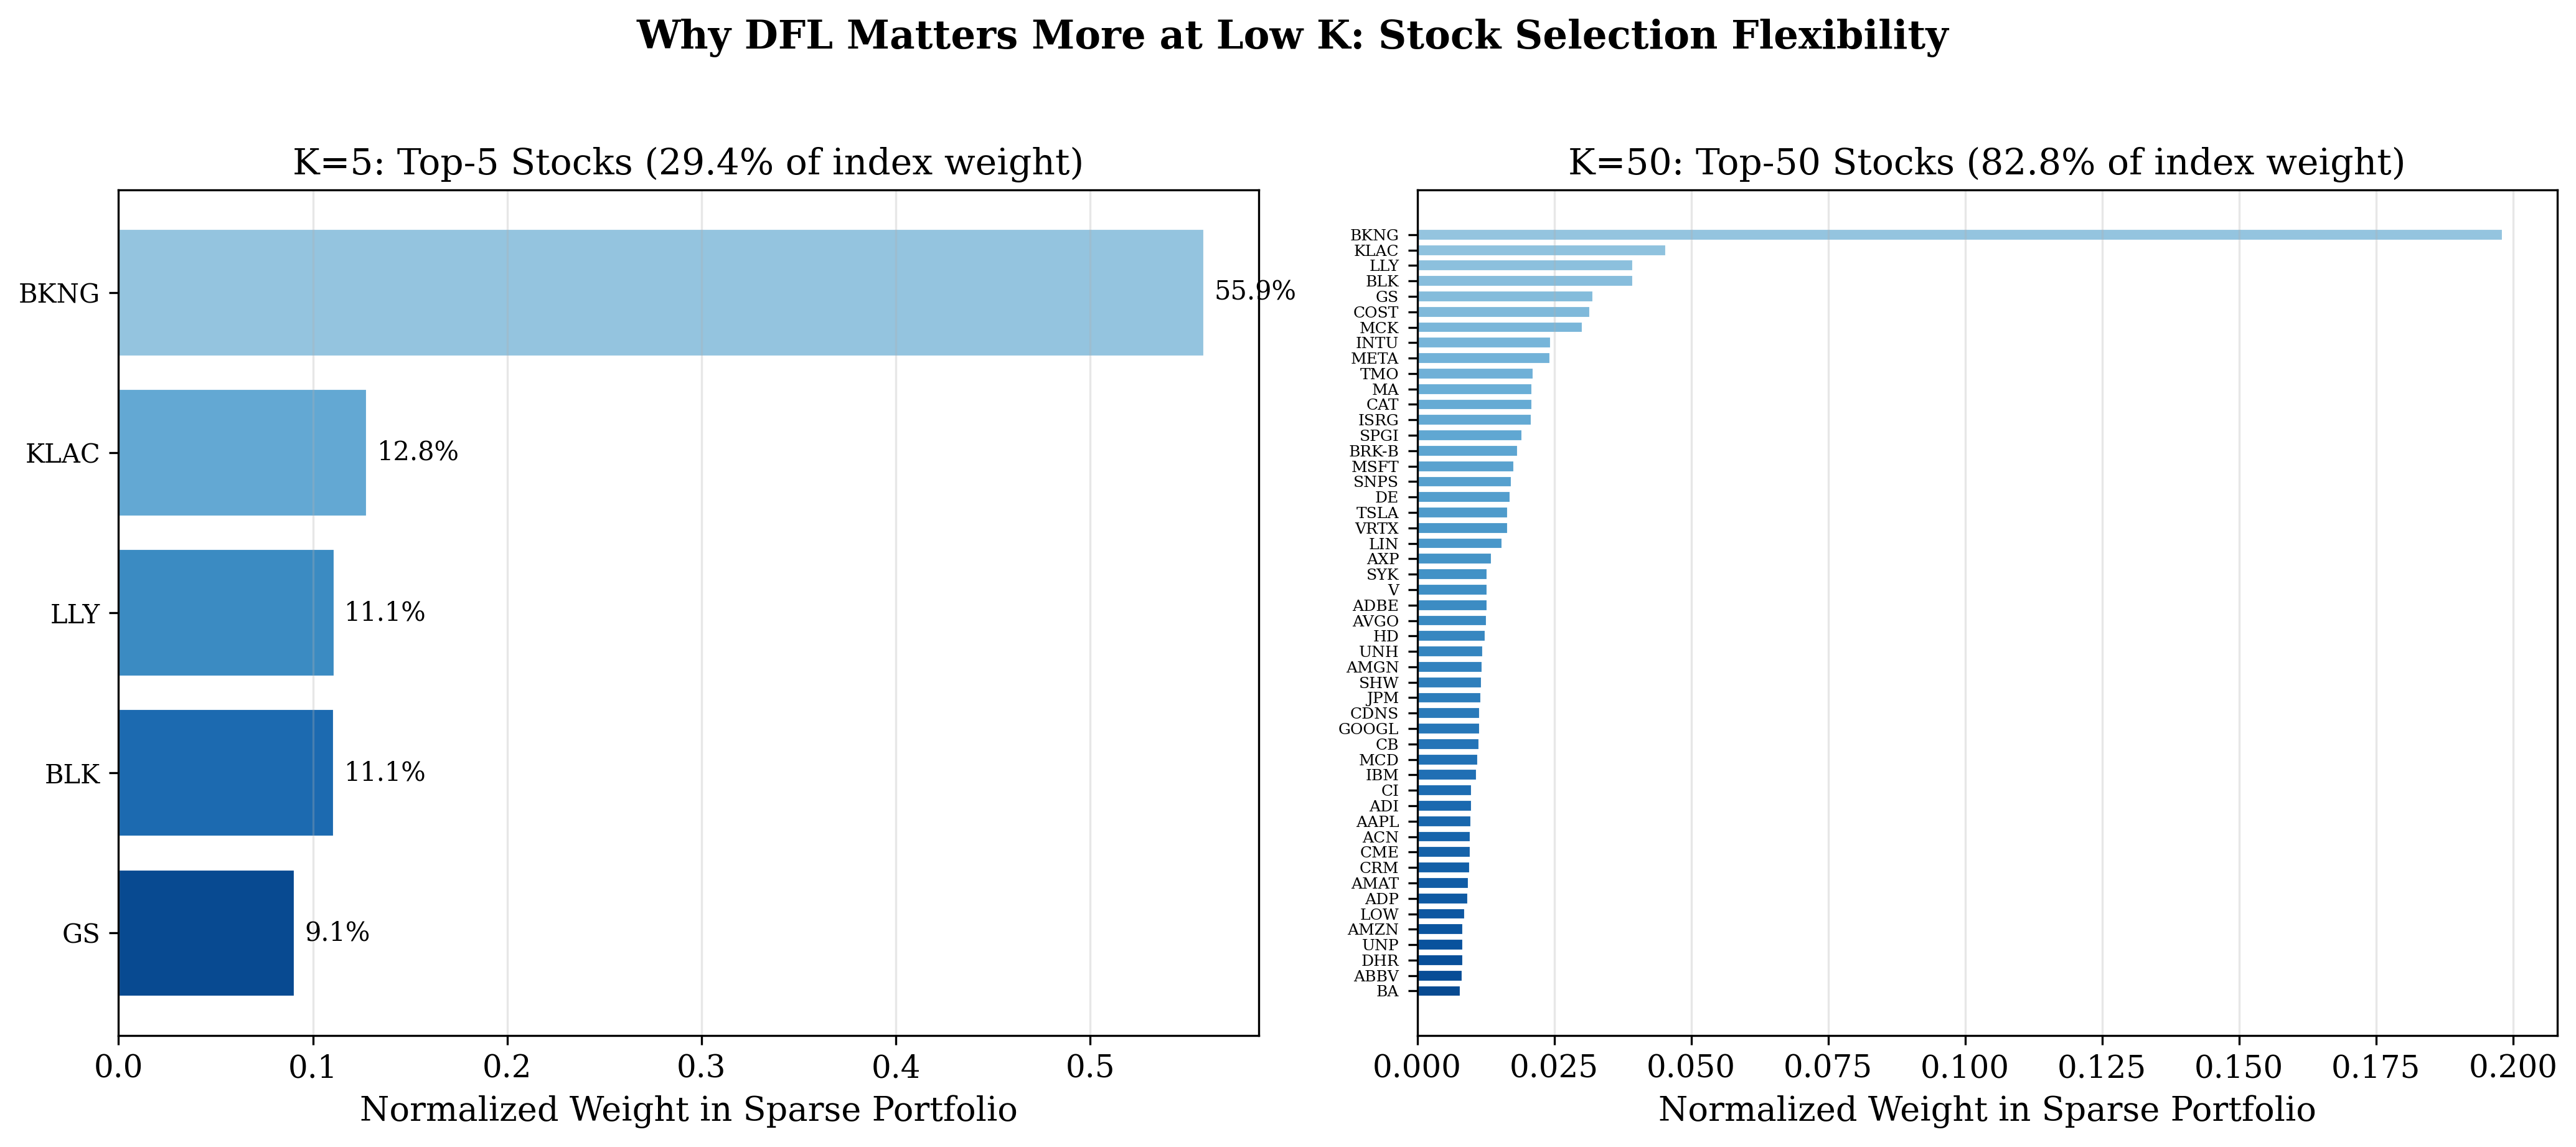
\includegraphics[width=0.95\textwidth]{../figures/fig7_selection_overlap.png}
\caption{Stock selection at $K = 5$ vs.\ $K = 50$. At low $K$, the QP solution is highly sensitive to covariance quality.}
\label{fig:selection}
\end{figure}

\subsection{Regime Analysis: DFL Shines in Volatile Markets}

We split test returns into three regimes based on rolling 21-day realized volatility of the index: \emph{Calm} ($< 33$rd percentile), \emph{Normal}, and \emph{Volatile} ($> 67$th percentile). Table~\ref{tab:regime} shows that DFL's advantage is largest in volatile markets — precisely when accurate covariance estimation matters most.

\begin{table}[H]
\centering
\caption{Neural+DFL vs.\ Neural+MSE tracking error by market regime. DFL's advantage is most pronounced in volatile conditions.}
\label{tab:regime}
\begin{tabular}{clccc}
\toprule
$K$ & Regime & Neural+DFL & Neural+MSE & $\Delta$ \\
\midrule
\multirow{3}{*}{5}
    & Calm     & 0.0687 & 0.0740 & $-7.3\%$  \\
    & Normal   & 0.0745 & 0.0811 & $-8.2\%$  \\
    & Volatile & 0.0931 & 0.1051 & $\mathbf{-11.4\%}$ \\
\midrule
\multirow{3}{*}{10}
    & Calm     & 0.0457 & 0.0494 & $-7.5\%$  \\
    & Normal   & 0.0462 & 0.0493 & $-6.3\%$  \\
    & Volatile & 0.0560 & 0.0593 & $-5.7\%$  \\
\midrule
\multirow{3}{*}{20}
    & Calm     & 0.0266 & 0.0299 & $-10.8\%$ \\
    & Normal   & 0.0274 & 0.0306 & $-10.4\%$ \\
    & Volatile & 0.0319 & 0.0369 & $\mathbf{-13.4\%}$ \\
\bottomrule
\end{tabular}
\end{table}

\begin{figure}[H]
\centering
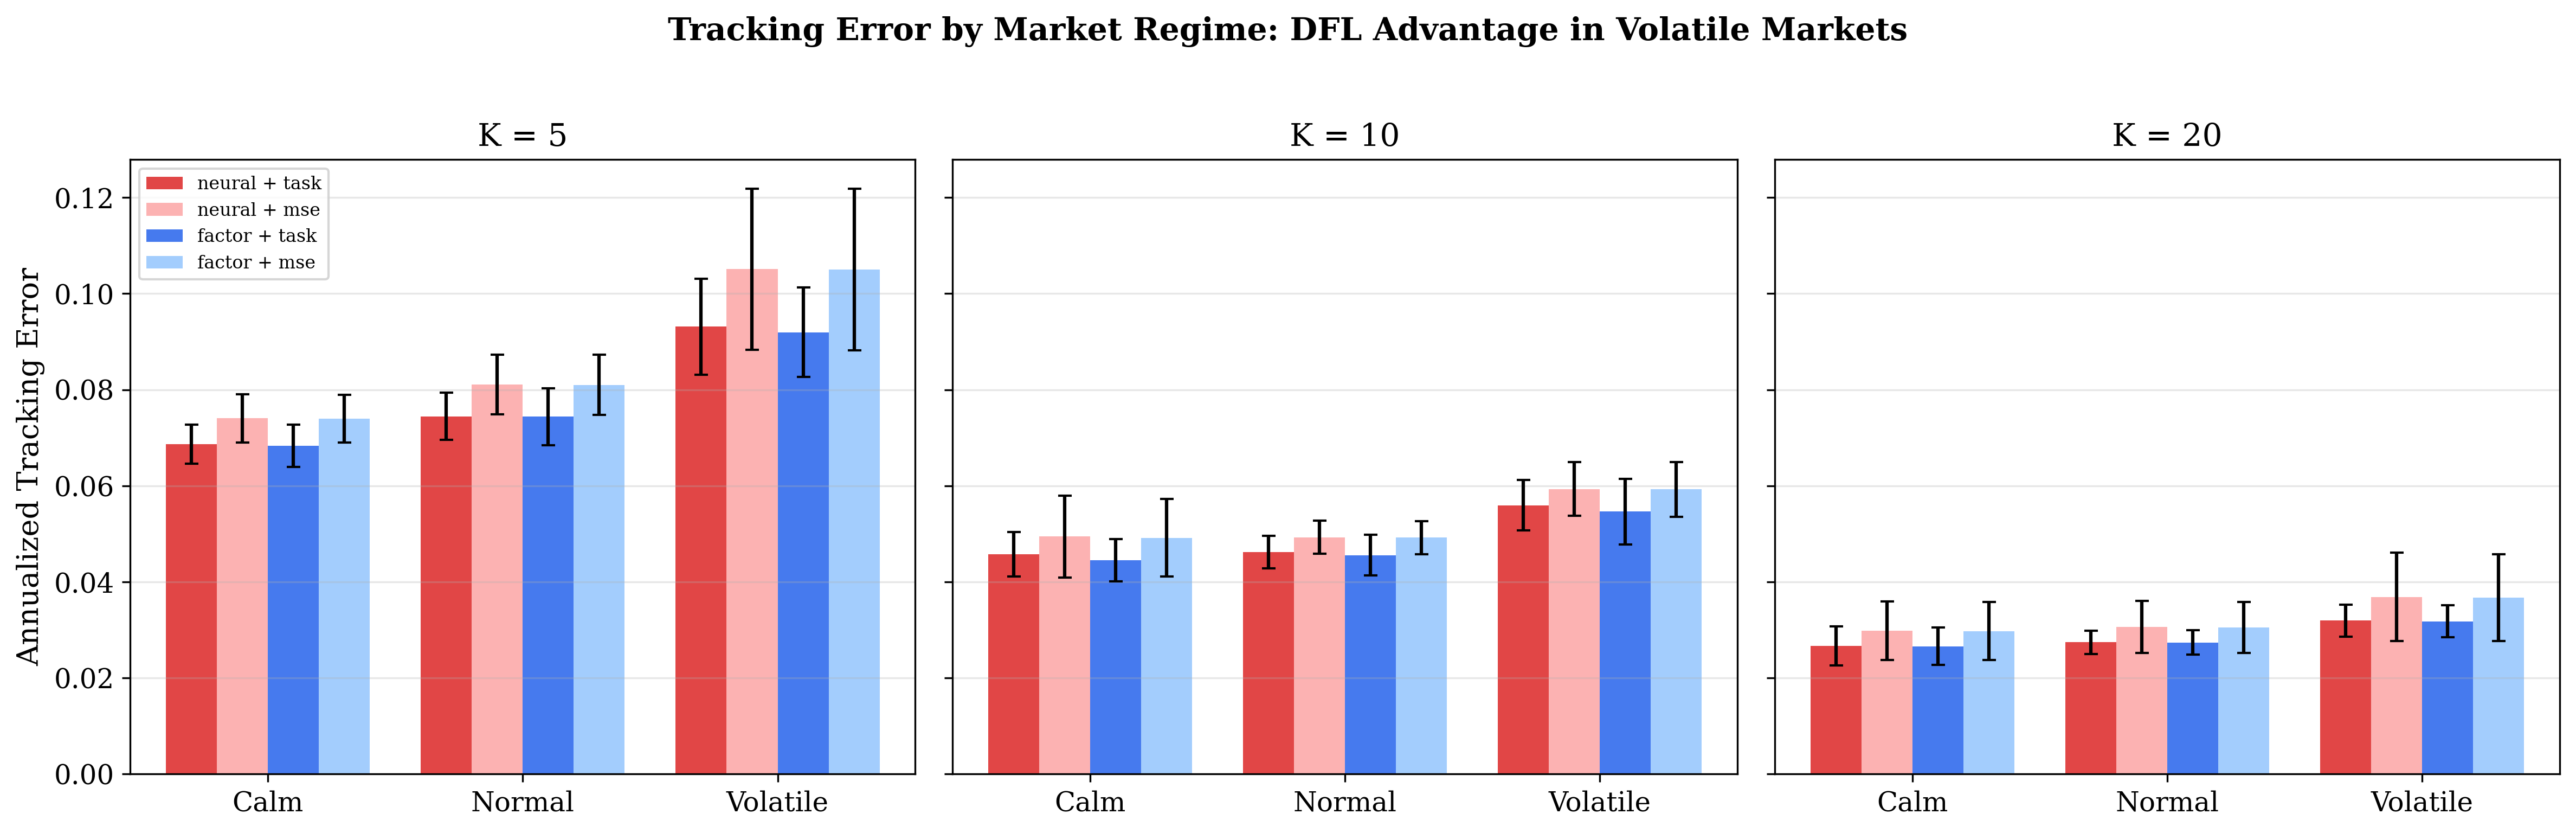
\includegraphics[width=0.95\textwidth]{../figures/fig9_regime_analysis.png}
\caption{Tracking error by market regime. DFL (darker bars) consistently outperforms MSE (lighter bars), with the largest gap in volatile markets.}
\label{fig:regime}
\end{figure}

\subsection{Turnover Analysis}

DFL models exhibit higher turnover than MSE baselines (Table~\ref{tab:turnover}), reflecting more active weight adjustments. However, we find that explicitly penalizing turnover ($\lambda > 0$) degrades tracking error — in the extreme, $\lambda = 0.1$ effectively freezes the neural model. The optimal setting is $\lambda = 0$ (no penalty), accepting higher turnover for better tracking.

\begin{table}[H]
\centering
\caption{Average turnover per rebalance. DFL has higher turnover but achieves lower tracking error.}
\label{tab:turnover}
\begin{tabular}{ccccc}
\toprule
$K$ & Neural+DFL & Neural+MSE & Factor+DFL & Factor+MSE \\
\midrule
5  & 0.042 & 0.003 & 0.056 & 0.001 \\
10 & 0.048 & 0.004 & 0.052 & 0.001 \\
20 & 0.030 & 0.003 & 0.051 & 0.001 \\
30 & 0.007 & 0.003 & 0.034 & 0.001 \\
50 & 0.001 & 0.001 & 0.021 & 0.001 \\
\bottomrule
\end{tabular}
\end{table}

\subsection{Cumulative Tracking Performance}

Figure~\ref{fig:cumulative} shows cumulative portfolio returns versus the index for the longest test fold at $K = 20$. DFL portfolios track the index more tightly, with smaller cumulative drift.

\begin{figure}[H]
\centering
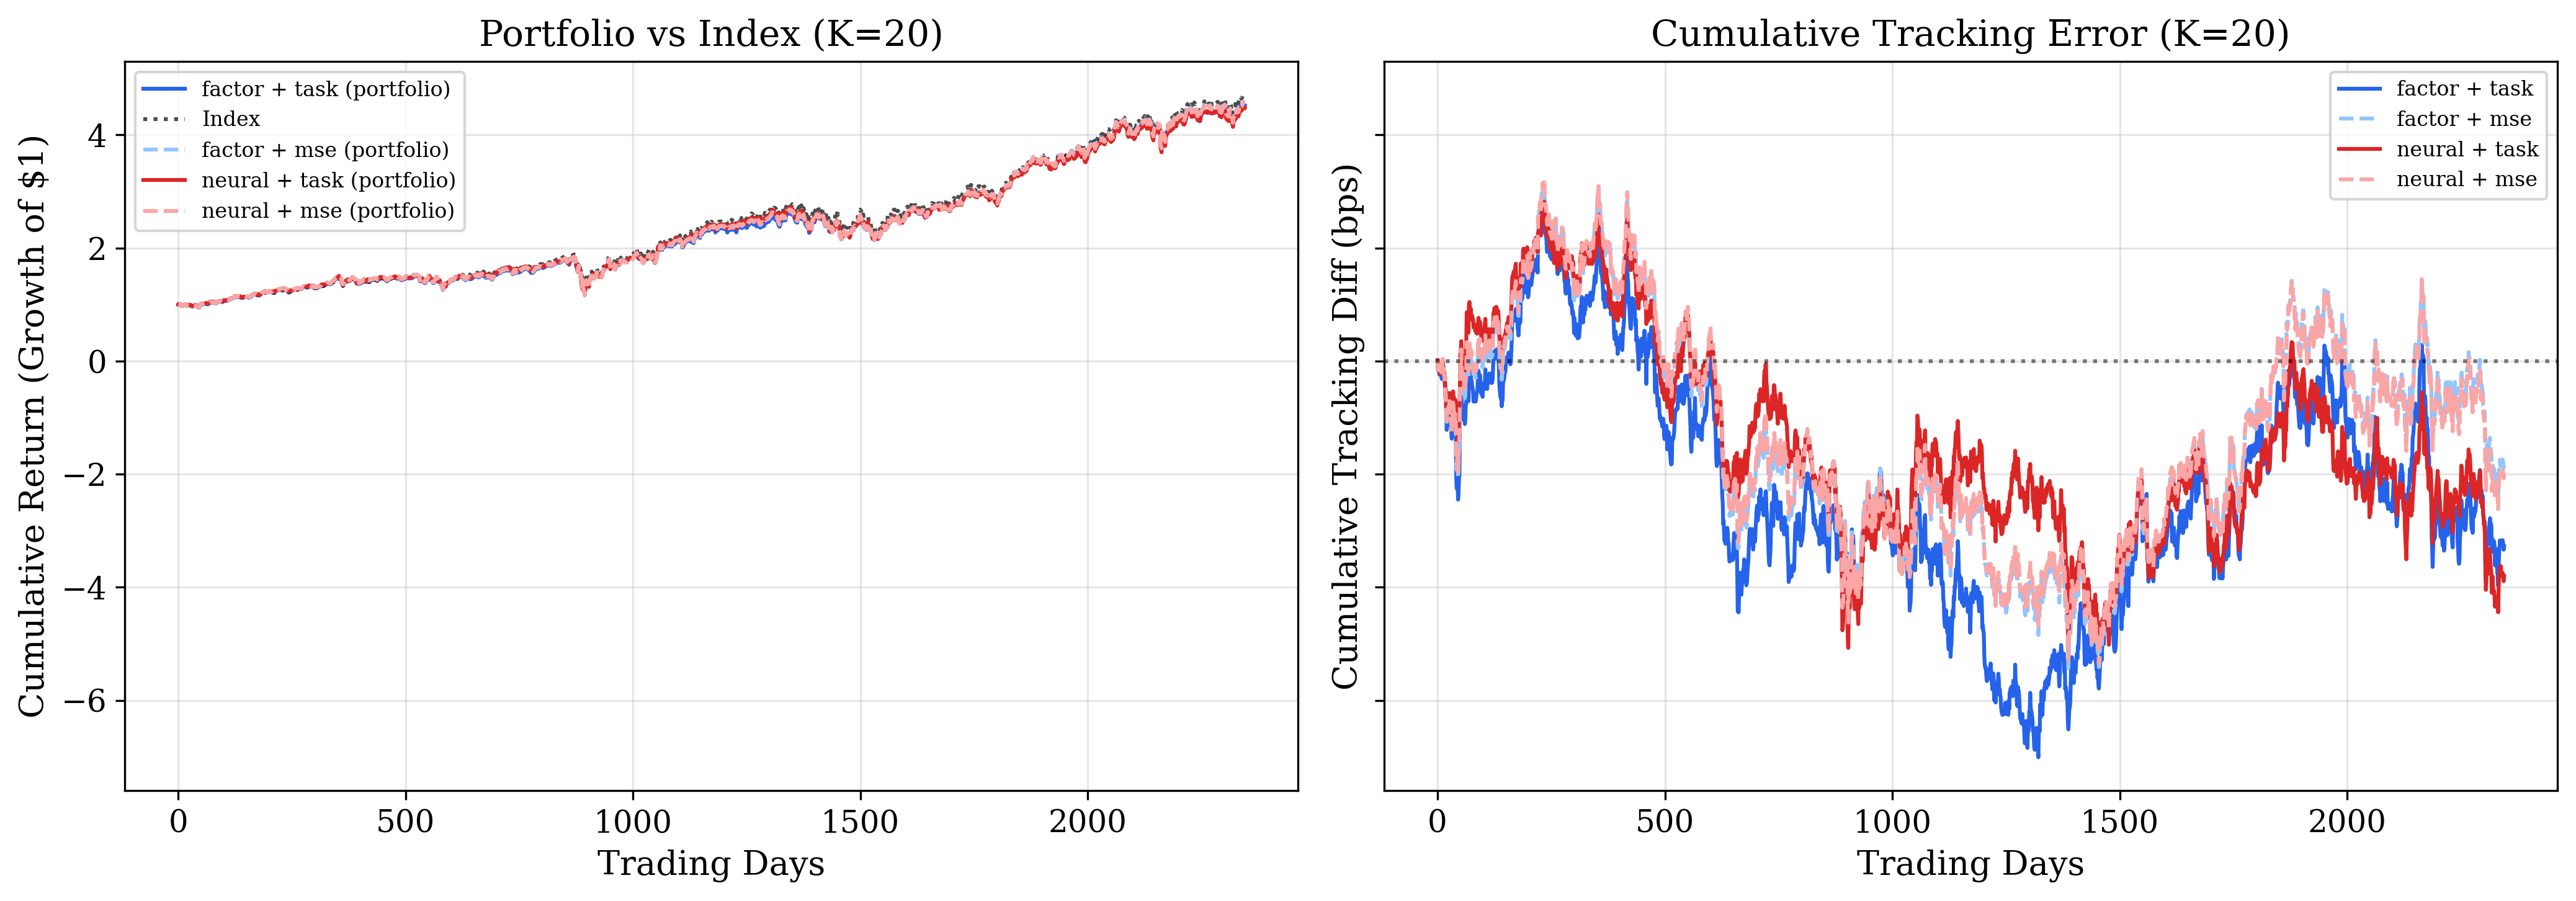
\includegraphics[width=0.95\textwidth]{../figures/fig5_cumulative_tracking_K20.png}
\caption{Cumulative portfolio return vs.\ index (left) and cumulative tracking difference (right) at $K = 20$.}
\label{fig:cumulative}
\end{figure}

% ══════════════════════════════════════════════════════════════════════
\section{Discussion}
\label{sec:discussion}

\paragraph{When does DFL help?}
Our results reveal a clear pattern: DFL provides the largest gains when (1) sparsity is tight ($K$ is small) and (2) markets are volatile. Both conditions amplify the sensitivity of the portfolio to covariance estimation quality. At high $K$ or in calm markets, even rough covariance estimates yield adequate portfolios, leaving little room for DFL to improve.

\paragraph{Factor vs.\ Neural.}
Both architectures benefit from DFL, with surprisingly similar improvements ($\sim$10\% at $K = 5, 20$). This suggests that the \emph{training objective} matters more than the \emph{model capacity} for this task. The factor model's low-rank inductive bias may even be advantageous — it prevents overfitting in the $O(N^2)$ covariance space.

\paragraph{Turnover--Tracking Error Trade-off.}
DFL achieves lower TE at the cost of higher turnover. In practice, this trade-off is managed by transaction cost budgets. We experimented with turnover penalties ($\lambda \in \{0, 0.01, 0.1\}$) but found that any $\lambda > 0$ disproportionately harms TE. Future work could explore adaptive penalty schedules.

\paragraph{Limitations.}
\begin{itemize}
    \item Stock selection is fixed by market-cap ranking, not learned. Covariance-aware selection could further amplify DFL's advantage but introduces combinatorial complexity.
    \item Transaction costs are not explicitly modeled beyond turnover measurement.
    \item The 97-stock universe is a subset of the full S\&P~500; larger universes may benefit more from DFL.
\end{itemize}

% ══════════════════════════════════════════════════════════════════════
\section{Conclusion}
\label{sec:conclusion}

We have demonstrated that Decision-Focused Learning significantly improves sparse index tracking at low sparsity levels. By replacing MSE with an end-to-end task loss that differentiates through a QP solver, our approach aligns the covariance model's training objective with the downstream portfolio decision. The key insight is that \emph{not all covariance errors are equal} — DFL focuses model capacity on the entries that matter for the portfolio, yielding up to 11.9\% tracking error reduction at $K = 20$. The advantage is robust across 9 rolling folds, two model architectures, and multiple market regimes, with the strongest gains in volatile conditions where accurate covariance estimation is most critical.

% ══════════════════════════════════════════════════════════════════════
\bibliographystyle{plainnat}
\begin{thebibliography}{10}

\bibitem[Agrawal et~al.(2019)]{agrawal2019differentiable}
Agrawal, A., Amos, B., Barratt, S., Boyd, S., Diamond, S., and Kolter, J.~Z.
\newblock Differentiable convex optimization layers.
\newblock In \emph{NeurIPS}, 2019.

\bibitem[Amos and Kolter(2017)]{amos2017optnet}
Amos, B. and Kolter, J.~Z.
\newblock OptNet: Differentiable optimization as a layer in neural networks.
\newblock In \emph{ICML}, 2017.

\bibitem[Beasley et~al.(2003)]{beasley2003evolutionary}
Beasley, J.~E., Meade, N., and Chang, T.-J.
\newblock An evolutionary heuristic for the index tracking problem.
\newblock \emph{European Journal of Operational Research}, 148(3):621--643, 2003.

\bibitem[Benidis et~al.(2018)]{benidis2018sparse}
Benidis, K., Feng, Y., and Palomar, D.~P.
\newblock Sparse portfolios for high-dimensional financial index tracking.
\newblock \emph{IEEE Transactions on Signal Processing}, 66(1):155--170, 2018.

\bibitem[Brodie et~al.(2009)]{brodie2009sparse}
Brodie, J., Daubechies, I., De~Mol, C., Giannone, D., and Loris, I.
\newblock Sparse and stable Markowitz portfolios.
\newblock \emph{PNAS}, 106(30):12267--12272, 2009.

\bibitem[Donti et~al.(2017)]{donti2017task}
Donti, P.~L., Amos, B., and Kolter, J.~Z.
\newblock Task-based end-to-end model learning in stochastic optimization.
\newblock In \emph{NeurIPS}, 2017.

\bibitem[Duchi et~al.(2008)]{duchi2008efficient}
Duchi, J., Shalev-Shwartz, S., Singer, Y., and Chandra, T.
\newblock Efficient projections onto the $\ell_1$-ball for learning in high dimensions.
\newblock In \emph{ICML}, 2008.

\bibitem[Elmachtoub and Grigas(2022)]{elmachtoub2022smart}
Elmachtoub, A.~N. and Grigas, P.
\newblock Smart ``predict, then optimize''.
\newblock \emph{Management Science}, 68(1):9--26, 2022.

\bibitem[Monga et~al.(2021)]{monga2021algorithm}
Monga, V., Li, Y., and Eldar, Y.~C.
\newblock Algorithm unrolling: Interpretable, efficient deep learning for signal and image processing.
\newblock \emph{IEEE Signal Processing Magazine}, 38(2):18--44, 2021.

\end{thebibliography}

\end{document}
